\subsubsection{Key derivation}
\label{sec:sphinx:keyderivation}

The sender $A$ picks a random $x\in \mathbb{Z}^*_q$ that is used to derive new keys for every packet.

$A$ randomly picks a path consisting of intermediate nodes $B$, $C$, $D$, and the packet's final destination, $Z$.

$A$ performs an offline Diffie-Hellman (DH) key exchange with each of these nodes and derives shared keys with each of them.

$A$ computes a sequence of tuples $(\alpha_i,s_i,b_i) \in \{ B, C, D, Z \}$ with $\alpha_A = g^x$ and $b_A = h_b(\alpha_A, s_B = y_B^{x b_A})$ as follows:

\begin{align}
    \nonumber(\alpha_B,s_B,b_B) & = (g^{x b_A},y_B^{x b_A},h_b(\alpha_B,s_B))                         \\
    \nonumber(\alpha_C,s_C,b_C) & = (g^{x b_A b_B},y_C^{x b_A b_B},h_b(\alpha_C,s_C))                 \\
    \nonumber(\alpha_D,s_D,b_D) & = (g^{x b_A b_B b_C},y_D^{x b_A b_B b_C},h_b(\alpha_D,s_D))         \\
    (\alpha_Z,s_Z,b_Z)          & = (g^{x b_A b_B b_C b_D},y_Z^{x b_A b_B b_C b_D},h_b(\alpha_Z,s_Z))
    \label{eq:1}
\end{align}
% % $$\alpha_0=g^x,s_0=y^x_B,b_0=h_b(a_0,s_0)$$
% and
% \begin{equation}
%     \begin{cases}
%         \alpha_i=g^{x\Pi_{j=0}^{j=i-2}b_j} \\
%         s_i=y^{x\Pi_{j=0}^{j=i-2}b_j}      \\
%         b_i=h_b(a_i,s_i)
%     \end{cases}\,.
%     \label{eq:1}
% \end{equation}
where $y_B, y_C, y_D$, and $y_Z$ are the public keys of the nodes $B, C, D$, and $Z$, respectively, which we assume to be available to $A$.

\begin{figure}[H]
    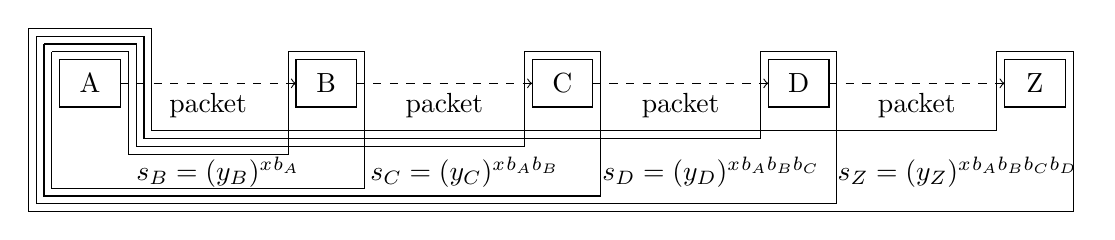
\begin{tikzpicture}
        \def\offset{3}
        \def\nodeWidth{0.77}
        \def\padding{0.93}
        \def\lowerpadding{0.7}
        \def\nodeHeight{0.6}
        \foreach \i\name\bi in{0/A/0,1/B/$^{b_A}$,2/C/$^{b_Ab_B}$,3/D/$^{b_Ab_Bb_C}$,4/Z/$^{b_Ab_Bb_Cb_D}$} {
                \draw (\i*\offset,0) rectangle (\i*\offset+\nodeWidth,\nodeHeight) node [midway] {\name};

                \ifnum\i>0
                    \draw (-0.1*\i,\nodeHeight+0.1*\i) -- (-0.1*\i,-\padding-0.1*\i) -- (\i*\offset+0.1+\nodeWidth,-\padding-0.1*\i) -- (\i*\offset+0.1+\nodeWidth,\nodeHeight+0.1) -- (\i*\offset-0.1,\nodeHeight+0.1) -- (\i*\offset-0.1,-\lowerpadding+0.1*\i) -- (\nodeWidth+0.1*\i,-\lowerpadding+0.1*\i) -- (\nodeWidth+0.1*\i,\nodeHeight+0.1*\i) -- (-0.1*\i,\nodeHeight+0.1*\i);
                \fi

                \ifnum\i>0
                    \draw [->,dashed] (\i*\offset-\offset+\nodeWidth,0.3) -- (\i*\offset,0.3) node [midway,below] {packet} node [midway,below=23pt,shift={(0.13*\i,0)}] {{\smaller$s_{\name}=(y_{\name})^x$\bi}};
                \fi
            }
    \end{tikzpicture}
    \caption{$A$ derives shared keys $s_B,s_C,s_D,s_Z$ with node $B,C,D,Z$ using their public keys $y_B,y_C,y_D,y_Z$.}
    \label{fig:sphinx:keyderivation}
\end{figure}